\vspace{1.5cm}

Es de esperarse que la fuente tenga un valor mínimo de tensión de entrada, a partir del cual empieza a regular la salida, para valores menores de tensión que este valor mínimo, la salida será menor a la esperada, en principio, el regulador paralelo para regular a $10 V$, necesita una tensión de entrada mayor, pero también se deben polarizar correctamente los transistores, y como puede verse en la figura~\figref{fig:fig_p18_vo_vs_vi}, el crecimiento de la salida es prácticamente lineal, manteniendo una diferencia de aproximadamente $2.4V$ a la salida con respecto a la entrada, este valor sería el \quotemarks{drop-out} de esta fuente de alimentación. Tomando que la salida está regulando al 
llegar a aproximadamente al $1 \%$ de la tensión regulada esperada a la salida, $10 V$, el valor de tensión de entrada mínimo para salida regulada es de $12.38 V$. También puede observarse que para tensiones muy pequeñas a la entrada, hasta aproximadamente $1.8 V$, la tensión a la salida es prácticamente $0 V$, esto se explica por estar cortado el elemento de paso de la fuente de alimentación, el par compuesto.

\vfill

\clearpage

\begin{figure}[H] %htb
\begin{center}
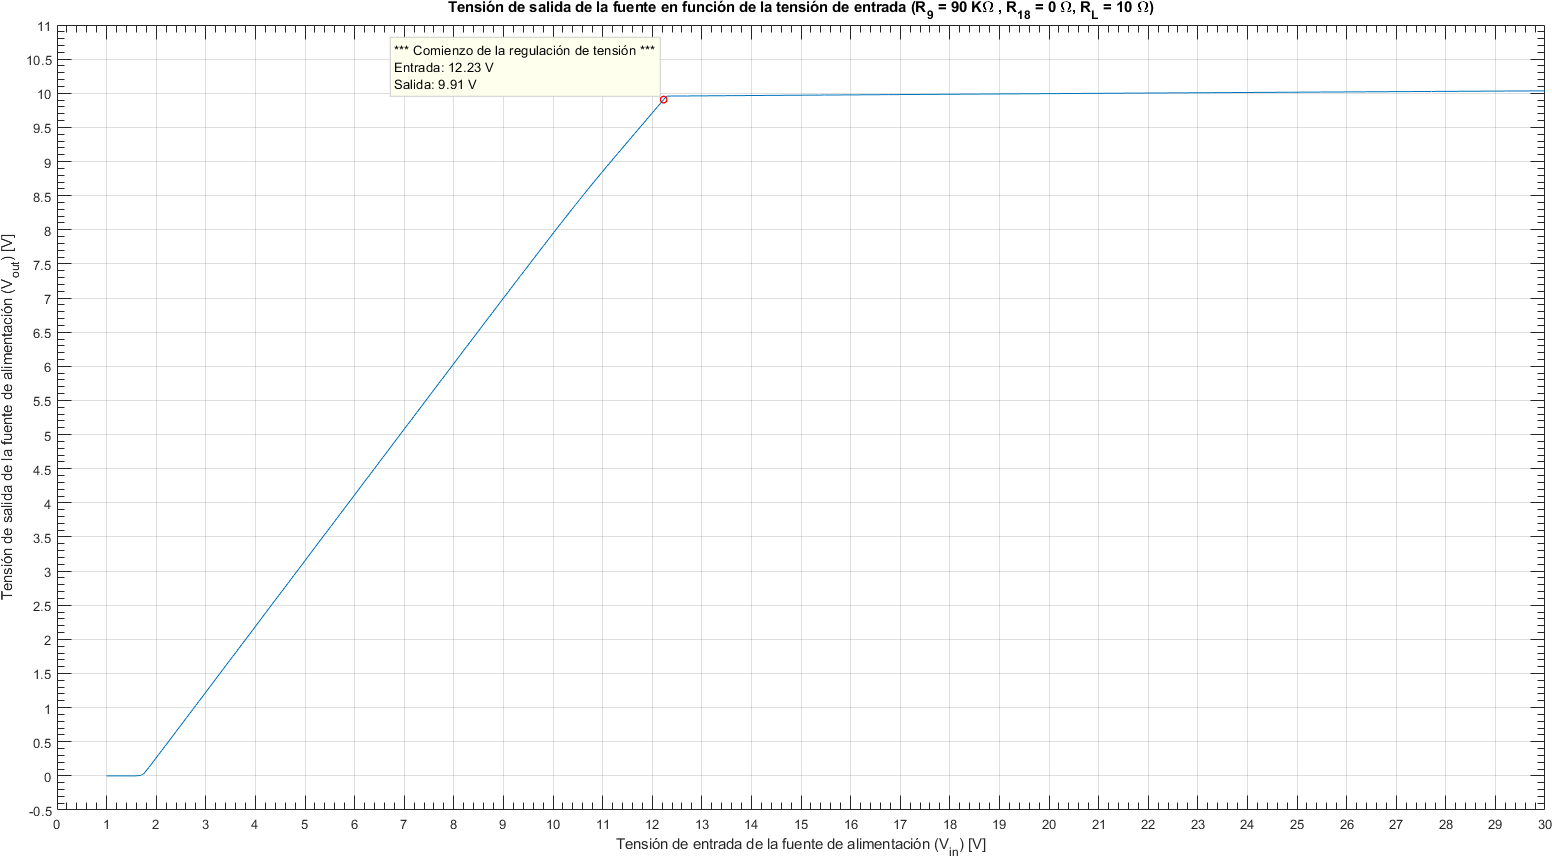
\includegraphics[width=1.2 \textwidth, angle=90]{./img/preguntas/p18.png}
\caption{\label{fig:fig_p18_vo_vs_vi}\footnotesize{Tensión de salida vs tensión de entrada.}}
\end{center}
\end{figure}

\clearpage